\documentclass[12pt,twoside,draft]{book}
\usepackage{../../thesis}
\graphicspath{ {../../images/} }
\usetikzlibrary{arrows,positioning} 
\tikzset{
    %Define standard arrow tip
    >=stealth',
    %Define style for boxes
    box/.style={
           rectangle,
           rounded corners,
           draw=black, very thick,
           text width=6.5em,
           minimum height=2em,
           text centered},
    % Define arrow style
    imply/.style={
           ->,
           thick,
           shorten <=2pt,
           shorten >=2pt},
    both/.style={
           <->,
           thick,
           shorten <=2pt,
           shorten >=2pt,},
    induced/.style={
           dotted,
           ->,
           thick,
           shorten <=2pt,
           shorten >=2pt},
    noimply/.style={
           ->,
           -o,
           thick,
           shorten <=2pt,
           shorten >=50pt}
}

\makeindex
\begin{document}
\chapter{Comparisons of Definitions of Chaos}
We have seen four definitions 
\begin{enumerate}[(i)]
  \item Devaney (\dev)
  \item Li-Yorke (\liy)
  \item Block-Coppel (\blcp)
  \item Positive topological entropy (\pte)
\end{enumerate}
and their variants
\begin{enumerate}[(i)]
  \item Wiggins's (similar to Devaney) (\wig)
  \item Martelli (equivalent to Wiggins's in $\R^n$)
  \item Marotto (implies Li-Yorke. Requires differentiability)
\end{enumerate}
In this chapter, we discuss the relations between the definitions (i)~(iv).
Throughout this chapter, we consider the dynamical system $(X,F)$, where $X$ is a compact metric space, and $F$ is a continuous mapping.
We first discuss a special case when $X$ is a compact interval, then proceed to the general case.
%%%

\section{Compact Interval}
Let $I \subseteq \R$ be a compact interval.
In this section, we consider the case where $X = I$.
As it turns out, Devaney's, Block-Coppel's, and positive topological entropy are equivalent conditions, and any of the three implies Li-Yorke's chaos.
\begin{figure}[ht]
  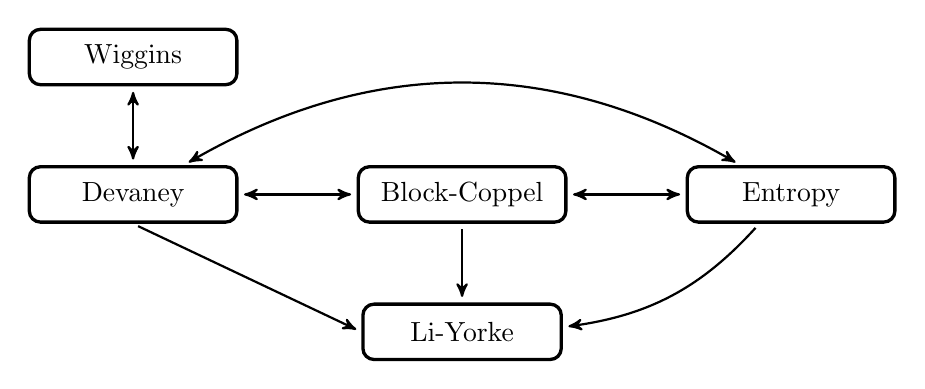
\begin{tikzpicture}[node distance=1cm, auto,]
 %nodes
    \node[box] (ly) {Li-Yorke};
    \node[box, inner sep=5pt,above=1.0cm of ly] (bc) {Block-Coppel};
    \node[box, inner sep=5pt,left=1.5cm of bc] (dev) {Devaney};
    \node[box, inner sep=5pt,right=1.5cm of bc] (ent) {Entropy};
    \node[box, inner sep=5pt,above=1.0cm of dev] (wig) {Wiggins};
 %edges
    \draw[imply] (dev.south) to node[bend right=20] {} (ly.west);  %this guy doesn't bend
    \draw[imply] (ent) to[bend left=20] node {} (ly); 
    \draw[imply] (bc) to node {} (ly); 
    \draw[both] (dev) to[bend left=30] node {} (ent); 
    \draw[both] (dev) to node {} (bc); 
    \draw[both] (dev) to node {} (wig); 
    \draw[both] (bc) to node {} (ent); 
  \end{tikzpicture}
  \label{fig:chaos-interval}
  \caption{
    Relations between the four definitions for the compact interval case.
    The three definitions in the top row are all equivalent.
    Li-Yorke's definition is strictly weaker than the other three.
  }
\end{figure}

\subsection*{Devaney and Block-Coppel}
We already mentioned in the chapter on Devaney's chaos that \dpp and \tt imply \sdic in a compact metric space.
Moreover, on a compact interval, topological transitivity implies the existence of dense periodic points.
Thus, Devaney's and Wiggins's definitions are equivalent.
\begin{theorem}
  $(I,F)$ is chaotic in the sense of Devaney if and only if it is chaotic in the sense of Wiggins.
  \label{thm:devaney-wiggins}
  \begin{proof}
    It follows from the fact that \tt implies \dpp on a compact interval.
    See \citet{silverman} for the proof.
  \end{proof}
\end{theorem}
Using the above result, we prove that \dev is equivalent to \blcp. 
\begin{theorem}
  \citep{aulbach}
  $(I,F)$ is chaotic in Devaney's sense if and only if it is chaotic in Block-Coppel's sense.
  \begin{proof}
    See \citep{aulbach}.
    The proof uses \citep{blockcoppel} VI: Proposition 6.
  \end{proof}
  \label{thm:devaney-blockcoppel}
\end{theorem}
%%%

\subsection*{Block-Coppel and Positive Topological Entropy}
Block-Coppel's definition is equivalent to a mapping having positive topological entropy.
\begin{theorem}
  $(I,F)$ is chaotic in the sense of Block-Coppel if and only if $F: I \to I$ has positive topological entropy.
  \label{thm:entropy-blockcoppel}
  \begin{proof}
    This follows from Theorem~\ref{thm:devaney-blockcoppel} and Theorem~\ref{thm:devaney-entropy}.
    It is also proved in \citet[VII, Theorem 24]{blockcoppel}.
  \end{proof}
\end{theorem}
Hence, the three definitions---Devaney, Block-Coppel, and positive topological entropy---are equivalent.
%%%

\subsection*{Block-Coppel and Li-Yorke}
Next, we show that Block-Coppel's definition implies Li-Yorke's definition.
\begin{theorem}
  \citep{blockcoppel}
  If $(I,F)$ is chaotic in Block-Coppel's sense, then it is chaotic in Li-Yorke's sense.
  \label{thm:devaney-liyorke}
  \begin{proof}
    See \citet{blockcoppel} (VI; Proposition 27).
  \end{proof}
\end{theorem}
The next example shows that the converse of the previous statement is not true in general.
\begin{example}
  \citep{blockcoppel}
  Truncated tent map.
  \label{eg:counterexample}
\end{example}

\subsection*{Result}
In summary, Devaney's, Block-Coppel's, and positive topological entropy definitions are equivalent on a compact interval.
Each of the three equivalent definitions imply chaos in Li-Yorke's sense, but Li-Yorke's definition does not imply others.
These results can be proved through other means.
\citet{smital} constructed an example of a Li-Yorke chaotic map that has zero topological entropy.
\citet{omegachaos} showed the equivalence of \dev and \pte, via his definition of chaos called $\omega$-chaos.
Also, some of these results are consequences of results in the general compact metric case.
%%%

\section{Compact Metric Space}
The result in this more general case is more interesting than the compact interval case.
\dev, \blcp, and \pte are no longer equivalent to each other.
Moreover, neither of them implies the others.
\begin{figure}[ht]
  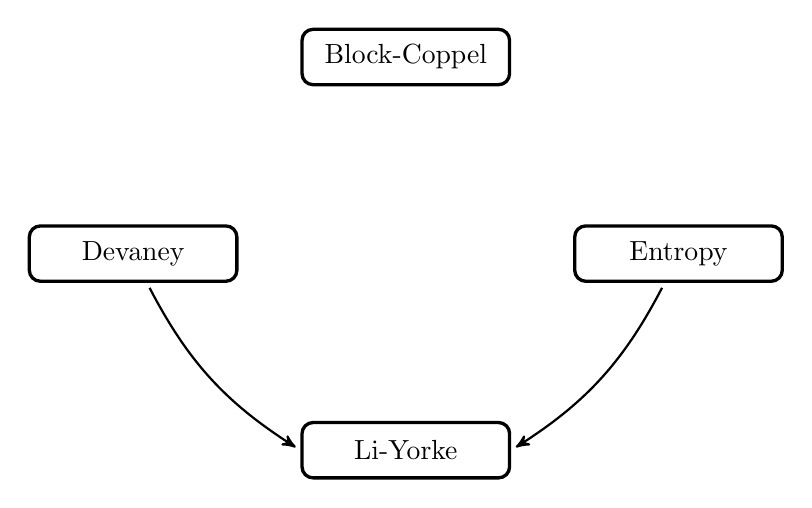
\begin{tikzpicture}[node distance=1cm, auto,]
 %nodes
    \node[] (dummy) {};
    \node[box, inner sep=5pt,below=2.0cm of dummy] (ly) {Li-Yorke};
    \node[box, inner sep=5pt,left=2.0cm of dummy] (dev) {Devaney};
    \node[box, inner sep=5pt,above=2.0cm of dummy] (bc) {Block-Coppel};
    \node[box, inner sep=5pt,right=2.0cm of dummy] (entropy) {Entropy};
 %edges
    \draw[imply] (entropy)[bend left=15] to node {} (ly.east); 
    \draw[imply] (dev)[bend right=15] to node {} (ly.west); 
    %? \draw[induced] (bc) to node {} (ly); 
    %? \draw[imply] (bc) to[bend left=15] node {} (entropy); 
    %??? \draw[imply] (bc) to[bend right=15] node {} (dev); 
  \end{tikzpicture}
  \label{fig:chaos-metric}
  \caption{
    Relations between definitions for a compact metric space.
    An absence of an arrow means that the particular implication is not necessarily true.
    For instance, Devaney's chaos does not imply Block-Copple's chaos.
  }
\end{figure}

\subsection*{Topological Entropy and Li-Yorke}
A system with posivite topological entropy is chaotic in Li-Yorke's sense.
\begin{theorem}
  \citep{blanchard}
  If $(X,F)$ has positive topological entropy, then it is chaotic in Li-Yorke's sense.
  \label{thm:entropy-liyorke}
\end{theorem}
As we have already seen in the compact interval case that the converse of the last theorem is not true in general.
For the same reason, LY implies neither Block-Coppel's nor Devaney's chaos.

\subsection*{Block-Coppel and Topological Entropy}
Even if $F$ is semi-conjugate to $\sigma$, we only have $h(F) \leq h(\sigma)$.
$h(\sigma)$ is positive, but we can't conclude that $h(F)$ is positive.

\subsection*{Block-Coppel and Devaney}
\citet{aulbach} has shown that Block-Coppel's definition does not imply Devaney's definition.
\begin{theorem}
  \citep{aulbach} 
  The adding machine is chaotic in Li-Yorke's sense \textit{and} in Block-Coppel's sense.
  However, the system is not chaotic in Devaney's sense.
  \begin{proof}
    (Adding machine example)
  \end{proof}
\end{theorem}
We do not know whether Block-Coppel implies Devaney.

\subsection*{Block-Coppel and Li-Yorke}
``it is widely believed that Block-Coppel implies Li-Yorke''

\subsection*{Devaney and Topological Entropy}

\subsection*{Devaney and Li-Yorke}
The following example is a system that is chaotic in Wiggins's sense but not in Li-Yorke's sense.
\begin{example}
  \citep{blanchard}
  Sturmian System.
  Chaos in Wiggins's sense is not a sufficient condition for chaos in Li-Yorke's sense.  
\end{example}
Obviously, this does not mean that Devaney's definition is not a sufficient condition for Li-Yorke's definition.
\citet{mai} proved that if a mapping is chaotic in Devaney's sense, then it is also chaotic in Li-Yorke's sense (\citet{huang} proved the same result earlier than Mai for the compact metric space case).
More specifically, Mai proved that, for a complete metric space $X$ without an isolated point, if $F: X \to X$ is transitive and has a periodic point of any period, then $F$ is chaotic in Li-Yorke's sense.
Thus, even though \tt and \sdic do not imply Li-Yorke's chaos, \tt and the existence of a single periodic points, which is significantly weaker than \dpp, imply chaos in Li-Yorke's sense.
We also notice that \sdic and the sensitivity conditions encoded in Li-Yorke's definition do not immediately imply each other.

\subsection*{Result}
There are open questions.

\bibliographystyle{../../bibliography/pjgsm}
\bibliography{../../bibliography/thesis}

\printindex
\end{document}

